\de{ĐỀ THI HỌC KỲ II NĂM HỌC 2022-2023}{Chuyên Lam Sơn-Thanh Hóa}

\begin{center}
	\textbf{PHẦN 1 - TRẮC NGHIỆM}
\end{center}
\Opensolutionfile{ans}[ans/ans]
\begin{ex}%[0D4B1-3]%[Dự án đề kiểm tra HKII-22-23,BCTuan]%[THPT Chuyên Lam Sơn-Thanh Hóa]
	\immini{
		Cho hàm số $y=f(x)=ax^2+bx+c$ có đồ thị như hình vẽ bên.\\
		Đặt $\Delta=b^2-4ac$, tìm dấu của $a$ và $\Delta$.
		\choice
		{$a<0$, $\Delta=0$}
		{$a<0$, $\Delta>0$}
		{\True $a>0$, $\Delta>0$}
		{$a>0$, $\Delta=0$}}
	{\vspace{-0.5cm}
		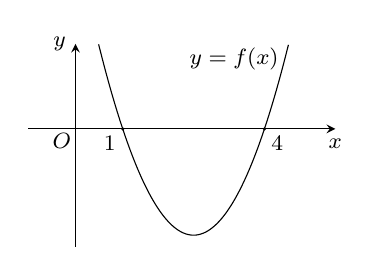
\begin{tikzpicture}[scale=0.6, font=\footnotesize, samples=200, >=stealth]
			\draw[->] (-1,0)--(5.5,0) node[below]{$x$};
			\draw[->] (0,-2.5)--(0,1.8) node[left]{$y$};
			\node at (0,0) [below left=-2pt]{$O$};
			\draw plot[domain=0.49:4.51](\x,{(\x)^2-5*\x+4}) node[left,yshift=-5]{$y=f(x)$};
			\fill
			(1,0) circle(1.07pt) node[below left=-1pt]{$1$}
			(4,0) circle(1.07pt) node[below right=-1pt]{$4$};
	\end{tikzpicture}}
	\loigiai{
		Parabol trong hình vẽ có bề lõm quay lên nên hệ số $a>0$.\\
		Parabol cắt trục hoành tại $2$ điểm phân biệt nên phương trình bậc hai $f(x)=0$ có $2$ nghiệm phân biệt, do đó $\Delta >0$.
	}
\end{ex}

\begin{ex}%[0D3Y2-3]%[Dự án đề kiểm tra HKII-22-23,BCTuan]%[THPT Chuyên Lam Sơn-Thanh Hóa]
	Cho hàm số bậc hai $y=ax^2+bx+c$ $(a \neq 0)$ có đồ thị $(P)$. Đỉnh của $(P)$ được xác định bởi công thức nào?
	\choice
	{$I\left(-\dfrac{b}{a};-\dfrac{\Delta}{4a}\right)$}
	{$I\left(-\dfrac{b}{2a};\dfrac{\Delta}{4a}\right)$}
	{\True $I\left(-\dfrac{b}{2a};-\dfrac{\Delta}{4a}\right)$}
	{$I\left(\dfrac{b}{2a};\dfrac{\Delta}{4a}\right)$}
	\loigiai{
		$I\left(-\dfrac{b}{2a};-\dfrac{\Delta}{4a}\right)$ là đỉnh của parabol $(P) \colon y=ax^2+bx+c$.
	}
\end{ex}

\begin{ex}%[0D3B1-2]%[Dự án đề kiểm tra HKII-22-23,BCTuan]%[THPT Chuyên Lam Sơn-Thanh Hóa]
	Trong các hàm số sau, hàm số nào có tập xác định là $\mathbb{R}$?
	\choice
	{$y=\dfrac{x+2}{x-1}$}
	{$y=\dfrac{x^2+2}{x}$}
	{$y=\dfrac{2x+3}{x^2}$}
	{\True $y=x^3+3x^2-1$}
	\loigiai{
		Hàm số $y=\dfrac{x+2}{x-1}$ có tập xác định $\mathbb{R} \setminus \{1\}$.\\
		Hàm số $y=\dfrac{x^2+2}{x}$ có tập xác định $\mathbb{R} \setminus \{0\}$.\\
		Hàm số $y=\dfrac{2x+3}{x^2}$ có tập xác định $\mathbb{R} \setminus \{0\}$.\\
		Hàm số $y=x^3+3x^2-1$ có tập xác định $\mathbb{R}$.
	}
\end{ex}

\begin{ex}%[0D3B2-2]%[Dự án đề kiểm tra HKII-22-23,BCTuan]%[THPT Chuyên Lam Sơn-Thanh Hóa]
	\immini{
		Bảng biến thiên như hình bên là bảng biến thiên của hàm số nào?
		\choice
		{\True $y=x^2+2x-2$}
		{$y=x^2-2x-2$}
		{$y=-x^2-2x-2$}
		{$y=x^2+3x-2$}}
	{\vspace{-0.5cm}
		
\begin{tikzpicture}
			\tkzTabInit[nocadre=true,lgt=1.2,espcl=2.5,deltacl=0.6]
			{$x$/0.6,$y$/2}
			{$-\infty$,$-1$,$+\infty$}
			\tkzTabVar{+/$+\infty$,-/$-3$,+/$+\infty$}
		\end{tikzpicture}
	}
	\loigiai{
		Bảng biến thiên thể hiện đồ thị hàm số có bề lõm quay lên nên $a>0$.\\
		Hoành độ đỉnh parabol là $x=-1$.\\
		Trong $4$ hàm số được cung cấp, chỉ có $y=x^2+2x-2$ có tính chất như thế.
	}
\end{ex}

\begin{ex}%[0H4Y3-1]%[Dự án đề kiểm tra HKII-22-23,BCTuan]%[THPT Chuyên Lam Sơn-Thanh Hóa]
	Elip $(E)\colon\dfrac{x^2}{16}+\dfrac{y^2}{9}=1$ có độ dài trục lớn bằng
	\choice
	{$9$}
	{$3$}
	{\True $8$}
	{$4$}
	\loigiai{
		Với $a^2=16$ ta có $a=4$, do đó độ dài trục lớn của $(E)$ là $2a=8$.
	}
\end{ex}

\begin{ex}%[0D4B1-2]%[Dự án đề kiểm tra HKII-22-23,BCTuan]%[THPT Chuyên Lam Sơn-Thanh Hóa]
	Cho tam thức $f(x)=ax^2+bx+c$ $(a \neq 0)$, $\Delta=b^2-4ac$. Ta có $f(x) \leq 0,\,\forall x \in \mathbb{R}$ khi và chỉ khi
	\def\dotEX{}
	\choice
	{$\heva{&a<0\\&\Delta \geq 0.}$}
	{\True $\heva{&a<0\\&\Delta \leq 0.}$}
	{$\heva{&a \leq 0\\&\Delta<0.}$}
	{$\heva{&a>0\\&\Delta \leq 0.}$}
	\loigiai{
		Với $f(x)=ax^2+bx+c$ $(a \neq 0)$, ta có $f(x) \leq 0,\,\forall x \in \mathbb{R}
		\Leftrightarrow \heva{&a<0\\&\Delta \leq 0.}$
	}
\end{ex}

\begin{ex}%[0D2K3-4]%[Dự án đề kiểm tra HKII-22-23,BCTuan]%[THPT Chuyên Lam Sơn-Thanh Hóa]
	Tổng $T=\mathrm{C}_n^0+\mathrm{C}_n^1+\mathrm{C}_n^2+\mathrm{C}_n^3+\mathrm{C}_n^4+ \cdots +\mathrm{C}_n^n$ bằng
	\choice
	{$2^{n-1}$}
	{$2^{n+1}$}
	{$0$}
	{\True $2^n$}
	\loigiai{
		Ta có $(1+x)^n=\mathrm{C}_n^0+\mathrm{C}_n^1\,x+\mathrm{C}_n^2\,x^2+\mathrm{C}_n^3\,x^3+\mathrm{C}_n^4\,x^4+ \cdots +\mathrm{C}_n^n\,x^n$.\\
		Thay $x=1$ ta được $2^n=\mathrm{C}_n^0+\mathrm{C}_n^1+\mathrm{C}_n^2+\mathrm{C}_n^3+\mathrm{C}_n^4+ \cdots +\mathrm{C}_n^n$ hay $T=2^n$.
	}
\end{ex}

\begin{ex}%[0D2Y1-1]%[Dự án đề kiểm tra HKII-22-23,BCTuan]%[THPT Chuyên Lam Sơn-Thanh Hóa]
	Trong một trường THPT, khối $11$ có $280$ học sinh nam và $325$ học sinh nữ. Nhà trường cần chọn một học sinh ở khối $11$ đi dự dạ hội của học sinh thành phố. Hỏi nhà trường có bao nhiêu cách chọn?
	\choice
	{\True $605$}
	{$45$}
	{$325$}
	{$280$}
	\loigiai{
		Do nhà trường chỉ cần chọn $1$ học sinh nên có $2$ phương án lựa chọn.\\
		Chọn $1$ nam, có $280$ cách; còn chọn $1$ nữ có $325$ cách.\\
		Theo quy tắc cộng, nhà trường có $280+325=605$ cách chọn.
	}
\end{ex}

\begin{ex}%[0H4B1-3]%[Dự án đề kiểm tra HKII-22-23,BCTuan]%[THPT Chuyên Lam Sơn-Thanh Hóa]
	Cho đường thẳng $d_1\colon 2x+3y+15=0$ và $d_2\colon x-2y-3=0$. Khẳng định nào sau đây đúng?
	\choice
	{$d_1$ và $d_2$ trùng nhau}
	{$d_1$ và $d_2$ vuông góc với nhau}
	{$d_1$ và $d_2$ song song với nhau}
	{\True $d_1$ và $d_2$ cắt nhau và không vuông góc với nhau}
	\loigiai{
		Ta có $d_1\colon 2x+3y+15=0$ và $d_2\colon x-2y-3=0$ có véc-tơ pháp tuyến lần lượt là 
		$$\vec{n}_{d_1}=(2;3) \text{ và } \vec{n}_{d_2}=(1;-2).$$
		Do $\heva{&\dfrac{2}{1} \neq \dfrac{3}{-2}\\&\vec{n}_{d_1} \cdot \vec{n}_{d_2}=-4 \neq 0}$ 
		nên $d_1$ và $d_2$ cắt nhau và không vuông góc với nhau.
	}
\end{ex}

\begin{ex}%[0D2Y2-8]%[Dự án đề kiểm tra HKII-22-23,BCTuan]%[THPT Chuyên Lam Sơn-Thanh Hóa]
	Kí hiệu $\mathrm{A}_n^k$ là số các chỉnh hợp chập $k$ của $n$ phần tử $(1 \leq k \leq n)$. Mệnh đề nào sau đây đúng?
	\choice
	{$\mathrm{A}_n^k=\dfrac{n!}{(n+k)!}$}
	{$\mathrm{A}_n^k=\dfrac{n!}{k!(n-k)!}$}
	{\True $\mathrm{A}_n^k=\dfrac{n!}{(n-k)!}$}
	{$\mathrm{A}_n^k=\dfrac{n!}{k!(n+k)!}$}
	\loigiai{
		$\mathrm{A}_n^k=\dfrac{n!}{(n-k)!}$.
	}
\end{ex}

\begin{ex}%[0D3Y2-9]%[Dự án đề kiểm tra HKII-22-23,BCTuan]%[THPT Chuyên Lam Sơn-Thanh Hóa]
	Cho $A$ là một biến cố liên quan phép thử $T$. Mệnh đề nào sau đây là mệnh đề đúng?
	\choice
	{$\mathrm{P}(A)$ là số lớn hơn $0$}
	{$\mathrm{P}(A)$ là số nhỏ hơn $1$}
	{\True $\mathrm{P}(A)=1-\mathrm{P}\left(\overline{A}\right)$}
	{$\mathrm{P}(A)=0 \Leftrightarrow A=\Omega$}
	\loigiai{
		Theo tính chất của hai biến cố đối nhau ta có $\mathrm{P}(A)=1-\mathrm{P}\left(\overline{A}\right)$.
	}
\end{ex}

\begin{ex}%[0H4B3-8]%[Dự án đề kiểm tra HKII-22-23,BCTuan]%[THPT Chuyên Lam Sơn-Thanh Hóa]
	Trong mặt phẳng tọa độ $Oxy$, phương trình nào là phương trình chính tắc của đường parabol?
	\choice
	{$x^2=6y$}
	{\True $y^2=6x$}
	{$y^2=-6x$}
	{$x^2=-6y$}
	\loigiai{
		$y^2=6x$ là phương trình chính tắc của đường parabol có tham số tiêu $p=3$.
	}
\end{ex}

\begin{ex}%[0H4B3-4]%[Dự án đề kiểm tra HKII-22-23,BCTuan]%[THPT Chuyên Lam Sơn-Thanh Hóa]
	Trong mặt phẳng tọa độ $Oxy$, cho hypebol có phương trình $\dfrac{x^2}{1}-\dfrac{y^2}{8}=1$. Tiêu cự hypebol bằng
	\choice
	{\True $6$}
	{$3$}
	{$1$}
	{$2\sqrt{7}$}
	\loigiai{
		Với $\heva{&a^2=1\\&b^2=8}$ ta có $c=\sqrt{a^2+b^2}=3$, từ đó tiêu cực của hypebol đã cho là $2c=6$.
	}
\end{ex}

\begin{ex}%[0D2Y3-1]%[Dự án đề kiểm tra HKII-22-23,BCTuan]%[THPT Chuyên Lam Sơn-Thanh Hóa]
	Trong khai triển nhị thức Niu-tơn của $(a+b)^4$ có bao nhiêu số hạng?
	\choice
	{\True $5$}
	{$4$}
	{$6$}
	{$3$}
	\loigiai{
		Trong khai triển nhị thức Niu-tơn của $(a+b)^4$ có $4+1=5$ số hạng.
	}
\end{ex}

\begin{ex}%[0H4Y1-1]%[Dự án đề kiểm tra HKII-22-23,BCTuan]%[THPT Chuyên Lam Sơn-Thanh Hóa]
	Cho đường thẳng $(d)\colon 3x+2y-10=0$. Véc-tơ nào sau đây là véc-tơ chỉ phương của $(d)$?
	\choice
	{$\vec{u}=(3;2)$}
	{$\vec{u}=(-2;-3)$}
	{\True $\vec{u}=(2;-3)$}
	{$\vec{u}=(3;-2)$}
	\loigiai{
		Đường thẳng $(d)\colon 3x+2y-10=0$ nhận $\vec{n}=(3;2)$ làm một véc-tơ pháp tuyến nên nhận $\vec{u}=(2;-3)$ làm một véc-tơ chỉ phương.
	}
\end{ex}

\begin{ex}%[0D3B1-2]%[Dự án đề kiểm tra HKII-22-23,BCTuan]%[THPT Chuyên Lam Sơn-Thanh Hóa]
	Không gian mẫu của phép thử ``\textit{gieo một con súc sắc $6$ mặt hai lần liên tiếp}'' có bao nhiêu phần tử?
	\choice
	{$12$}
	{\True $36$}
	{$24$}
	{$30$}
	\loigiai{
		Phép thử ``\textit{gieo một con súc sắc $6$ mặt hai lần liên tiếp}'' có $6^2=36$ phần tử.
	}
\end{ex}

\begin{ex}%[0D3Y1-2]%[Dự án đề kiểm tra HKII-22-23,BCTuan]%[THPT Chuyên Lam Sơn-Thanh Hóa]
	Tập xác định $\mathscr{D}$ của hàm số $y=\sqrt{3x-1}$ là
	\choice
	{$\mathscr{D}=(0;+\infty)$}
	{$\mathscr{D}=[0;+\infty)$}
	{$\mathscr{D}=\left(\dfrac{1}{3};+\infty\right)$}
	{\True $\mathscr{D}=\left[\dfrac{1}{3};+\infty\right)$}
	\loigiai{
		Điều kiện xác định của hàm số $y=\sqrt{3x-1}$ là $3x-1 \geq 0 \Leftrightarrow x \geq \dfrac{1}{3}$.\\
		Tập xác định của hàm số là $\mathscr{D}=\left[\dfrac{1}{3};+\infty\right)$.
	}
\end{ex}

\begin{ex}%[0D4B2-1]%[Dự án đề kiểm tra HKII-22-23,BCTuan]%[THPT Chuyên Lam Sơn-Thanh Hóa]
	Tập nghiệm của bất phương trình $2x^2-14x+20<0$ là
	\choice
	{$S=(-\infty;2) \cup (5;+\infty)$}
	{$S=(-\infty;2] \cup [5;+\infty)$}
	{$S=[2;5]$}
	{\True $S=(2;5)$}
	\loigiai{
		Cho $2x^2-14x+20=0 \Leftrightarrow \hoac{&x=2\\&x=5.}$\\
		Bảng xét dấu
		\begin{center}
			\begin{tikzpicture}
				\tkzTabInit[nocadre=true,lgt=3.7,espcl=2,deltacl=0.6]
				{$x$/0.6,$2x^2-14x+20$/0.6}
				{$-\infty$,$2$,$5$,$+\infty$}
				\tkzTabLine{,+,$0$,-,$0$,+,}
			\end{tikzpicture}
		\end{center}
		Tập nghiệm của bất phương trình $2x^2-14x+20<0$ là $S=(2;5)$.
	}
\end{ex}

\begin{ex}%[0D2Y2-2]%[Dự án đề kiểm tra HKII-22-23,BCTuan]%[THPT Chuyên Lam Sơn-Thanh Hóa]
	Số cách chọn $5$ học sinh trong một lớp có $25$ học sinh nam và $16$ học sinh nữ là
	\choice
	{$\mathrm{C}_{25}^5+\mathrm{C}_{16}^5$}
	{$\mathrm{A}_{41}^5$}
	{\True $\mathrm{C}_{41}^5$}
	{$\mathrm{C}_{25}^5$}
	\loigiai{
		Số cách chọn $5$ học sinh trong một lớp có $25$ học sinh nam và $16$ học sinh nữ là $\mathrm{C}_{25+16}^5$.
	}
\end{ex}

\begin{ex}%[0H4B2-1]%[Dự án đề kiểm tra HKII-22-23,BCTuan]%[THPT Chuyên Lam Sơn-Thanh Hóa]
	Trong mặt phẳng $Oxy$, đường tròn $(C)\colon x^2+y^2+4x+6y-12=0$ có tâm là
	\choice
	{$I(2;3)$}
	{\True $I(-2;-3)$}
	{$I(-4;-6)$}
	{$I(4;6)$}
	\loigiai{
		Đường tròn $(C)\colon x^2+y^2+4x+6y-12=0$ có tâm $I(-2;-3)$.
	}
\end{ex}

\begin{ex}%[0H4B3-5]%[Dự án đề kiểm tra HKII-22-23,BCTuan]%[THPT Chuyên Lam Sơn-Thanh Hóa]
	Trong mặt phẳng tọa độ $Oxy$, phương trình chính tắc của hypebol $(H)$ có một tiêu điểm $F(5;0)$ và độ dài trục thực bằng $8$ là
	\choice
	{\True $\dfrac{x^2}{16}-\dfrac{y^2}{9}=1$}
	{$\dfrac{x^2}{16}+\dfrac{y^2}{9}=1$}
	{$\dfrac{x^2}{16}-\dfrac{y^2}{9}=-1$}
	{$\dfrac{x^2}{9}-\dfrac{y^2}{16}=1$}
	\loigiai{
		Hypebol $(H)$ có một tiêu điểm $F(5;0)$ và độ dài trục thực bằng $8$ nên 
		$$\heva{&c=5\\&2a=8} \Leftrightarrow \heva{&a^2+b^2=c^2=25\\&a^2=16} \Leftrightarrow \heva{&b^2=9\\&a^2=16.}$$
		Phương trình của hypebol là $\dfrac{x^2}{16}-\dfrac{y^2}{9}=1$.
	}
\end{ex}

\begin{ex}%[0H4B1-2]%[Dự án đề kiểm tra HKII-22-23,BCTuan]%[THPT Chuyên Lam Sơn-Thanh Hóa]
	Phương trình tham số của đường thẳng $d$ đi qua điểm $M(4;-7)$ và song song với trục hoành là
	\def\dotEX{}
	\choice
	{$\heva{&x=4+t\\&y=-7.}$}
	{\True $\heva{&x=4\\&y=-7+t.}$}
	{$\heva{&x=-7+t\\&y=4.}$}
	{$\heva{&x=1+4t\\&y=-7t.}$}
	\loigiai{
		Đường thẳng $d$ đi qua điểm $M(4;-7)$ và song song với trục hoành nhận $\vec{i}=(1;0)$ làm một véc-tơ chỉ phương, do đó $d$ có phương trình tham số là $\heva{&x=4\\&y=-7+t.}$
	}
\end{ex}

\begin{ex}%[0D4B1-2]%[Dự án đề kiểm tra HKII-22-23,BCTuan]%[THPT Chuyên Lam Sơn-Thanh Hóa]
	Tam thức nào dưới đây luôn dương với mọi giá trị của $x \in \mathbb{R}$?
	\choice
	{$x^2-2x-10$}
	{$x^2-10x+2$}
	{\True $x^2-2x+10$}
	{$-x^2+2x+10$}
	\loigiai{
		Ta có $x^2-2x+10=x^2-2x+1+9=(x-1)^2+9>0,\,\forall x \in \mathbb{R}$.
	}
\end{ex}

\begin{ex}%[0D2B3-3]%[Dự án đề kiểm tra HKII-22-23,BCTuan]%[THPT Chuyên Lam Sơn-Thanh Hóa]
	Khai triển $\left(1+2x+3x^2\right)^{10}=a_0+a_1x+a_2x^2+ \cdots +a_{20}x^{20}$. Tính tổng $S=a_0+2a_1+4a_2+ \cdots +2^{20}a_{20}$.
	\choice
	{$S=15^{10}$}
	{\True $S=17^{10}$}
	{$S=7^{10}$}
	{$S=17^{20}$}
	\loigiai{
		Với $\left(1+2x+3x^2\right)^{10}=a_0+a_1x+a_2x^2+ \cdots +a_{20}x^{20}$, cho $x=2$ ta được
		$$\left(1+2\cdot 2+3\cdot 2^2\right)^{10}=a_0+a_1\cdot 2+a_2\cdot 2^2+ \cdots +a_{20}\cdot 2^{20} \Leftrightarrow S=17^{10}.$$
	}
\end{ex}

\begin{ex}%[0D4B1-2]%[Dự án đề kiểm tra HKII-22-23,BCTuan]%[THPT Chuyên Lam Sơn-Thanh Hóa]
	Các giá trị của tham số $m$ để tam thức $f(x)=x^2-(m+2)x+6m+1$ đổi dấu $2$ lần là
	\choice
	{\True $m<0$ hoặc $m>20$}
	{$m \leq 0$ hoặc $m \geq 20$}
	{$m>0$}
	{$0<m<20$}
	\loigiai{
		Tam thức $f(x)=x^2-(m+2)x+6m+1$ đổi dấu $2$ lần khi và chỉ khi 
		$$\begin{aligned}
			\Delta_f=(m+2)^2-4(6m+1)>0 
			& \Leftrightarrow m^2-20m>0\\
			& \Leftrightarrow m \in (-\infty;0) \cup (20;+\infty).
		\end{aligned}$$
	}
\end{ex}

\begin{ex}%[0D2B2-4]%[Dự án đề kiểm tra HKII-22-23,BCTuan]%[THPT Chuyên Lam Sơn-Thanh Hóa]
	Đa giác lồi $10$ cạnh có bao nhiêu đường chéo?
	\choice
	{$10$}
	{$45$}
	{$20$}
	{\True $35$}
	\loigiai{
		Số đoạn thẳng có $2$ đầu mút lấy từ $2$ trong $10$ đỉnh của đa giác lồi $10$ cạnh là $\mathrm{C}_{10}^2$.\\
		Trong các đoạn thẳng nêu trên có $10$ đoạn thẳng là cạnh (không phải đường chéo) của đa giác lồi đã cho, do đó số đường chéo của đa giác lồi đã cho là $\mathrm{C}_{10}^2-10=35$.
	}
\end{ex}

\begin{ex}%[0D3B2-4]%[Dự án đề kiểm tra HKII-22-23,BCTuan]%[THPT Chuyên Lam Sơn-Thanh Hóa]
	Một hộp chứa ba quả cầu trắng và hai quả cầu đen. Lấy ngẫu nhiên đồng thời hai quả cầu. Xác suất để lấy được cả hai quả cầu trắng là
	\choice
	{$\dfrac{4}{10}$}
	{\True $\dfrac{3}{10}$}
	{$\dfrac{2}{10}$}
	{$\dfrac{5}{10}$}
	\loigiai{
		Lấy ngẫu nhiên đồng thời hai quả cầu từ hộp chứa $3$ quả cầu trắng và $2$ quả cầu đen, số kết quả có thể xảy ra là $n(\Omega)=\mathrm{C}_5^2=10$.\\
		Xét biến cố $A$: ``lấy được $2$ quả cầu trắng''.\\
		Số kết quả thuận lợi cho $A$ là $n(A)=\mathrm{C}_3^2=3$, do đó $\mathrm{P}(A)=\dfrac{n(A)}{n(\Omega)}=\dfrac{3}{10}$.
	}
\end{ex}

\begin{ex}%[0D2B3-2]%[Dự án đề kiểm tra HKII-22-23,BCTuan]%[THPT Chuyên Lam Sơn-Thanh Hóa]
	Trong khai triển biểu thức $(x+y)^{21}$, hệ số của số hạng chứa $x^{13}y^8$ là
	\choice
	{$293930$}
	{$1287$}
	{$116280$}
	{\True $203490$}
	\loigiai{
		Số hạng tổng quát trong khai triển của $(x+y)^{21}$ có dạng $\mathrm{C}_{21}^k\,x^{21-k}y^k$ $(k \in \mathbb{N},\, k \leq 21)$.\\
		Số hạng chứa $x^{13}y^8$ ứng với $k=8$, do đó hệ số cần tìm là $\mathrm{C}_{21}^8=203490$.
	}
\end{ex}

\begin{ex}%[0D3B1-5]%[Dự án đề kiểm tra HKII-22-23,BCTuan]%[THPT Chuyên Lam Sơn-Thanh Hóa]
	\immini{
		Cho hàm số có đồ thị như hình bên. Khẳng định nào sau đây là đúng?
		\choice
		{Hàm số nghịch biến trên khoảng $(0;3)$}
		{Hàm số đồng biến trên khoảng $(-\infty;3)$}
		{Hàm số đồng biến trên khoảng $(-\infty;1)$}
		{\True Hàm số nghịch biến trên khoảng $(0;2)$}}
	{\vspace{-0.5cm}
		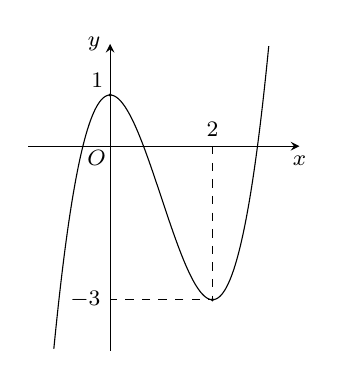
\begin{tikzpicture}[scale=0.65, font=\footnotesize, samples=200, >=stealth]
			\draw[->] (-1.6,0)--(3.7,0) node[below]{$x$};
			\draw[->] (0,-4)--(0,2) node[left]{$y$};
			\node at (0,0) [below left=-2pt]{$O$};
			\draw plot[domain=-1.1:3.1] (\x,{(\x)^3-3*(\x)^2+1});
			\fill
			(0,1) circle(1pt) node[above left=-1pt]{$1$}
			(2,-3) circle(1pt);
			\draw[dashed]
			(2,0) node[above]{$2$} |-(0,-3)node[left]{$-3$};
	\end{tikzpicture}}
	\loigiai{
		Hình bên có đồ thị của hàm số đồng biến trên các khoảng $(-\infty;0)$, $(2;+\infty)$ và nghịch biến trên khoảng $(0;2)$.
	}
\end{ex}

\begin{ex}%[0D2B1-5]%[Dự án đề kiểm tra HKII-22-23,BCTuan]%[THPT Chuyên Lam Sơn-Thanh Hóa]
	Từ các chữ số $1$, $5$, $6$, $7$ có thể lập được bao nhiêu chữ số tự nhiên có $4$ chữ số?
	\choice
	{$124$}
	{\True $256$}
	{$248$}
	{$324$}
	\loigiai{
		Xét số $\overline{abcd}$ với $a,b,c,d \in \big\{1;5;6;7\big\}$.\\
		Số cách chọn cho mỗi vị trí $a,b,c,d$ là $4$.\\
		Do đó số cách chọn được $1$ số thỏa mãn yêu cầu bài toán là $4\cdot 4\cdot 4\cdot 4=256$.
	}
\end{ex}


\begin{ex}%[0D2B3-2]%[Dự án đề kiểm tra HKII NH22-23- Phạm Phương]%[THPT CHUYÊN LAM SƠN - THANH HÓA]
	Hệ số của số hạng chứa $x^3$ trong khai triển thành đa thức của biểu thức $A=(1-x)^{10}$ là
	\choice
	{\True $-120$}
	{$120$}
	{$-30$}
	{$30$}
	\loigiai{
		Số hạng tổng quát trong khai triển của $(1-x)^{10}$ có dạng $\mathrm{C}_{10}^k\,(-x)^k=\mathrm{C}_{10}^k\,(-1)^k\,x^k$ $(k \in \mathbb{N},\, k \leq 10)$.\\
		Số hạng chứa $x^3$ ứng với $k=3$, do đó hệ số cần tìm là $\mathrm{C}_{10}^3\,(-1)^3=-120$.
	}
\end{ex}

\begin{ex}%[0H4B3-8]%[Dự án đề kiểm tra HKII NH22-23- Phạm Phương]%[THPT CHUYÊN LAM SƠN - THANH HÓA]
	Trong mặt phẳng tọa độ $Oxy$, phương trình nào sau đây là phương trình chính tắc của parabol nhận $F\left(\dfrac{9}{2};0\right)$ làm tiêu điểm
	\choice
	{$y=9x^2$}
	{\True $y^2=18x$}
	{$y^2=9x$}
	{$y=18x^2$}
	\loigiai{
		Parabol nhận $F\left(\dfrac{9}{2};0\right)$ làm tiêu điểm có tham số tiêu $p$ thỏa mãn $\dfrac{p}{2}=\dfrac{9}{2} \Leftrightarrow p=9$.\\
		Phương trình chính tắc của hypebol đó là $y^2=2px \Leftrightarrow y^2=18x$.
	}
\end{ex}

\begin{ex}%[0D2B2-4]%[Dự án đề kiểm tra HKII NH22-23- Phạm Phương]%[THPT CHUYÊN LAM SƠN - THANH HÓA]
	Cho đa giác đều có $20$ đỉnh. Số tam giác được tạo thành từ các đỉnh của đa giác là
	\choice
	{\True $\mathrm{C}_{20}^3$}
	{$2!\mathrm{C}_{20}^3$}
	{$\mathrm{A}_{20}^3$}
	{$10^3$}
	\loigiai{
		Mỗi tam giác được tạo thành từ các đỉnh của đa giác đều $20$ cạnh là một tổ hợp chập $3$ của $20$ phần tử, do đó số tam giác cần đếm là $\mathrm{C}_{20}^3$.
	}
\end{ex}

\begin{ex}%[0D3K2-3]%[Dự án đề kiểm tra HKII NH22-23- Phạm Phương]%[THPT CHUYÊN LAM SƠN - THANH HÓA]
	\immini{
		Cho hàm số $y=ax^2+bx+c$ có đồ thị là parabol trong hình vẽ bên. Khẳng định nào sau đây đúng?
		\choice
		{\True $a>0$, $b>0$, $c<0$}
		{$a>0$, $b>0$, $c>0$}
		{$a>0$, $b<0$, $c>0$}
		{$a>0$, $b<0$, $c<0$}}
	{\vspace{-0.5cm}
		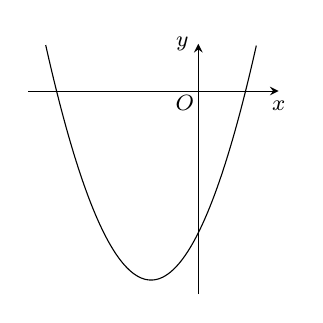
\begin{tikzpicture}[scale=0.6, font=\footnotesize, samples=200, >=stealth]
			\draw[->] (-3.6,0)--(1.7,0) node[below]{$x$};
			\draw[->] (0,-4.3)--(0,1) node[left]{$y$};
			\node at (0,0) [below left=-2pt]{$O$};
			\draw plot[domain=-3.23:1.23](\x,{(\x)^2+2*\x-3});
	\end{tikzpicture}}
	\loigiai{
		Pababol trong hình vẽ có bề lõm quay lên nên $a>0$, cắt trục hoành tại điểm $A(0;c)$ phía dưới $O$ nên $c<0$.\\
		Ngoài ra trục đối xứng của parabol $x=-\dfrac{b}{2a}$ nằm bên trái trục tung nên $b$ và $a$ cùng dấu nhau, do đó $b>0$.\\
		Vậy $a>0$, $b>0$, $c<0$.
	}
\end{ex}

\begin{ex}%[0H4B1-4]%[Dự án đề kiểm tra HKII NH22-23- Phạm Phương]%[THPT CHUYÊN LAM SƠN - THANH HÓA]
	Cho hai đường thẳng $d_1\colon 2x+5y-2=0$ và $d_2\colon 3x-7y+3=0$. Góc tạo bởi đường thẳng $d_1$ và $d_2$ bằng
	\choice
	{$60^{\circ}$}
	{$135^{\circ}$}
	{\True $45^{\circ}$}
	{$30^{\circ}$}
	\loigiai{
		Gọi $\alpha$ là góc giữa $d_1\colon 2x+5y-2=0$ và $d_2\colon 3x-7y+3=0$, ta có
		$$\cos\alpha=\dfrac{\big|2\cdot 3+5\cdot(-7)\big|}{\sqrt{2^2+5^2}\cdot\sqrt{3^2+(-7)^2}}=\dfrac{\sqrt{2}}{2} 
		\Rightarrow \alpha = 45^{\circ}.$$
	}
\end{ex}

\begin{ex}%[0D3Y2-1]%[Dự án đề kiểm tra HKII NH22-23- Phạm Phương]%[THPT CHUYÊN LAM SƠN - THANH HÓA]
	Gieo ngẫu nhiên một con súc sắc. Xác suất để mặt $6$ chấm xuất hiện là
	\choice
	{$\dfrac{1}{2}$}
	{$\dfrac{1}{3}$}
	{$\dfrac{5}{6}$}
	{\True $\dfrac{1}{6}$}
	\loigiai{
		Xác suất để mặt $6$ chấm xuất hiện khi gieo một con súc sắc $6$ mặt là $\dfrac{1}{6}$.
	}
\end{ex}

\begin{ex}%[0D4B3-2]%[Dự án đề kiểm tra HKII NH22-23- Phạm Phương]%[THPT CHUYÊN LAM SƠN - THANH HÓA]
	Phương trình $\sqrt{3x+4}=x$ có tập nghiệm là
	\choice
	{$S=\{-1\}$}
	{\True $S=\{4\}$}
	{$S=\varnothing$}
	{$S=\{-1;4\}$}
	\loigiai{
		Ta có $\sqrt{3x+4}=x \Rightarrow 3x+4=x^2 \Leftrightarrow x^2-3x-4=0 \Leftrightarrow \hoac{&x=-1\\&x=4.}$\\
		Lần lượt thay $x=-1$ và $x=4$ vào phương trình $\sqrt{3x+4}=x$ ta thấy chỉ có $x=4$ thỏa mãn phương trình.\\
		Vậy phương trình đã cho có tập nghiệm $S=\{4\}$.
	}
\end{ex}

\begin{ex}%[0D3K1-2]%[Dự án đề kiểm tra HKII NH22-23- Phạm Phương]%[THPT CHUYÊN LAM SƠN - THANH HÓA]
	Tìm các giá trị thực của tham số $m$ để hàm số $y=\dfrac{x+m+2}{x-m}$ xác định trên $(-1;3)$.
	\def\dotEX{}
	\choice
	{$-1<m<3$.}
	{$\hoac{&m<-1\\&m>3.}$}
	{\True $\hoac{&m \leq -1\\&m \geq 3.}$}
	{$\heva{&m \leq -1\\&m \geq 3.}$}
	\loigiai{
		Điều kiện xác định của $y=\dfrac{x+m+2}{x-m}$ là $x \neq m$.\\
		Do đó hàm số xác định trên khoảng $(-1;3)$ khi và chỉ khi $m \notin (-1;3) \Leftrightarrow \hoac{&m \leq -1\\&m \geq 3.}$
	}
\end{ex}

\begin{ex}%[0H4B2-5]%[Dự án đề kiểm tra HKII NH22-23- Phạm Phương]%[THPT CHUYÊN LAM SƠN - THANH HÓA]
	Trong mặt phẳng tọa độ $Oxy$, phương trình của đường tròn có tâm là gốc tọa độ $O$ và tiếp xúc với đường thẳng $\Delta\colon x+y-2=0$ là
	\choice
	{$(x-1)^2+(y-1)^2=\sqrt{2}$}
	{\True $x^2+y^2=2$}
	{$(x-1)^2+(y-1)^2=2$}
	{$x^2+y^2=\sqrt{2}$}
	\loigiai{
		Đường tròn $(C)$ có tâm $O(0;0)$ và tiếp xúc với $\Delta\colon x+y-2=0$ có bán kính là $$R=\mathrm{d}(O,\Delta)=\dfrac{|0+0-2|}{\sqrt{1^2+1^2}}=\sqrt{2}.$$
		Từ đó phương trình đường tròn $(C)\colon x^2+y^2=2$.
	}
\end{ex}

\begin{ex}%[0H4K3-1]%[Dự án đề kiểm tra HKII NH22-23- Phạm Phương]%[THPT CHUYÊN LAM SƠN - THANH HÓA]
	Cho elip $(E)\colon\dfrac{x^2}{25}+\dfrac{y^2}{9}=1$. Trong các khẳng định sau, khẳng định nào \textbf{sai}?
	\choice
	{\True $(E)$ có độ dài trục nhỏ bằng $3$}
	{$(E)$ có các tiêu điểm $F_1(-4;0)$ và $F_2(4;0)$}
	{$(E)$ có đỉnh $A_1(-5;0)$}
	{$(E)$ có tỉ số $\dfrac{c}{a}=\dfrac{4}{5}$}
	\loigiai{
		Elip $(E)\colon\dfrac{x^2}{25}+\dfrac{y^2}{9}=1$ có $\heva{&a^2=25\\&b^2=9} \Leftrightarrow \heva{&a=5\\&b=3}$, suy ra $c=\sqrt{a^2-b^2}=4$.\\
		Do đó $(E)$ có độ dài trục nhỏ $2b=6$; $A_1(-5;0)$ là một đỉnh; hai tiêu điểm $F_1(-4;0)$, $F_2(4;0)$ và tỉ số $\dfrac{c}{a}=\dfrac{4}{5}$.\\
		Vậy khẳng định ``$(E)$ có độ dài trục nhỏ bằng $3$'' là sai.
	}
\end{ex}

\begin{ex}%[0D2K1-3]%[Dự án đề kiểm tra HKII NH22-23- Phạm Phương]%[THPT CHUYÊN LAM SƠN - THANH HÓA]
	Cho tập hợp $A=\{0;1;2;3;5\}$. Từ tập $A$ có thể lập được bao nhiêu số chia hết cho $5$ gồm $4$ chữ số khác nhau?
	\choice
	{$54$}
	{$72$}
	{$69$}
	{\True $42$}
	\loigiai{
		Xét số $\overline{abcd} \;\vdots\; 5$, với $a,b,c,d$ khác nhau lấy từ $A=\{0;1;2;3;5\}$. Khi đó $d=0$ hoặc $d=5$.\\
		\begin{itemize}
			\item Nếu $d=0$ ta xét số $\overline{abc0}$, với $a,b,c \in \{1;2;3;5\}$.\\
			Số cách chọn $a,b,c$ khác nhau (theo thứ tự đó) là $4,3,2$.\\
			Trường hợp này có $4\cdot 3\cdot 2=24$ số.
			\item Nếu $d = 5$ ta xét số $\overline{abc5}$, với $a,b,c \in \{0;1;2;3\}$, $a \neq 0$.\\
			Số cách chọn $a,b,c$ khác nhau (theo thứ tự đó) là $3,3,2$.\\
			Trường hợp này có $3\cdot 3\cdot 2=18$ số.
		\end{itemize}
		Vậy có $24+18=42$ số thỏa mãn yêu cầu của bài toán.
	}
\end{ex}

\begin{ex}%[0D4K2-1]%[Dự án đề kiểm tra HKII NH22-23- Phạm Phương]%[THPT CHUYÊN LAM SƠN - THANH HÓA]
	Có bao nhiêu giá trị nguyên của tham số $m$ để hàm số $y=\sqrt{x^2-2mx-2m+3}$ có tập xác định là $\mathbb{R}$.
	\choice
	{\True $5$}
	{$3$}
	{$4$}
	{$6$}
	\loigiai{
		Hàm số $y=\sqrt{x^2-2mx-2m+3}$ có tập xác định là $\mathbb{R}$ khi và chỉ khi 
		$$\begin{aligned}
			x^2-2mx-2m+3 \geq 0,\;\forall x\in \mathbb{R}
			&\Leftrightarrow \Delta'=m^2+2m-3 \leq 0
			&\Leftrightarrow -3 \leq m \leq 1.
		\end{aligned}$$
		Chỉ xét $m \in \mathbb{Z}$ ta nhận $m \in \{-3;-2;-1;0;1\}$ (có $5$ giá trị $m$).
	}
\end{ex}

\begin{ex}%[0D3G2-5]%[Dự án đề kiểm tra HKII NH22-23- Phạm Phương]%[THPT CHUYÊN LAM SƠN - THANH HÓA]
	\immini{
		Cổng Arch tại thành phố St.Louis của Mỹ có hình dạng là một parabol. Biết khoảng cách giữa hai chân cổng bằng $162 \mathrm{\,m}$. Trên thành cổng, tại vị trí có độ cao $43 \mathrm{\,m}$ so với mặt đất, người ta thả một sợi dây chạm đất. Vị trí chạm đất của đầu sợi dây này cách chân cổng $A$ một đoạn $10 \mathrm{\,m}$. Giả sử các số liệu trên là chính xác. Hãy tính độ cao của cổng Arch (chính xác đến phần chục)?
		\choice
		{$175{,}6 \mathrm{\,m}$}
		{$197{,}5 \mathrm{\,m}$}
		{$210 \mathrm{\,m}$}
		{\True $185{,}6 \mathrm{\,m}$}}
	{\vspace{-0.5cm}
		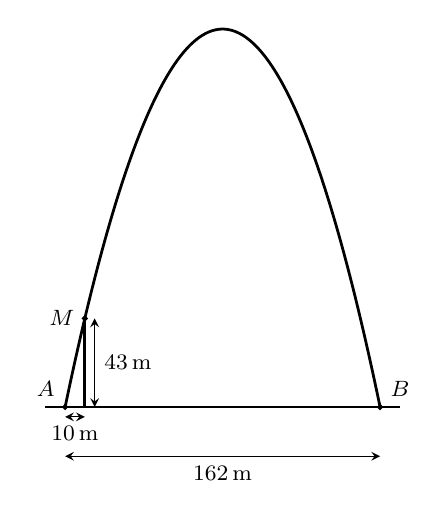
\begin{tikzpicture}[scale=0.25,line width=1pt,>=stealth,x=1mm,y=1mm]
			\draw (-10,0)--(0,0) node[above left] {\footnotesize $A$} -- (160,0) node[above right]{\footnotesize $B$}--(170,0) (10,45) node[left]{\footnotesize $M$};
			\draw(10,0)--(10,45);
			\draw[<->,thin](15,0)--(15,45) node[midway,right]{\footnotesize $43 \mathrm{\,m}$};
			\draw[<->,thin] (0,-5)--(10,-5) node[midway,below]{\footnotesize $10 \mathrm{\,m}$};
			\draw[<->,thin] (0,-25)--(160,-25)node[midway,below]{\footnotesize $162 \mathrm{\,m}$};
			\draw[fill=black](0,0) circle (2pt) (10,45) circle (2pt) (160,0) circle (2pt); 
			\usepgflibrary{fpu}
			\draw[smooth,samples=100,domain=0:160,/pgf/fpu,/pgf/fpu/output format=fixed] plot(\x,{-0.03*(\x)^2+4.8*(\x)});
	\end{tikzpicture}}
	\loigiai{
		\immini{
			Đặt hệ trục toạ độ với $Axy$ như hình vẽ.\\
			Xét parabol $(P)\colon\,y=ax^2+bx+c$.\\
			Vì $M(10;43) \in (P)$ nên $100a+10b+c=43$.\hfill($ 1 $)\\
			Vì $A(0;0) \in (P)$ nên $c=0$.\hfill($ 2 $)\\
			Vì $B(162;0) \in (P)$ nên $162^2a+162b+c=0$.\hfill($ 3 $)\\
			Giải hệ ($ 1 $), ($ 2 $), ($ 3 $) ta được $(P)\colon y=-\dfrac{43}{1520}x^2+\dfrac{3483}{760}x$.\\
			$(P)$ có trục đối xứng là $x=81$.\\
			Suy ra chiều cao của cổng là $y(81) \approx 185{,}607 \mathrm{\,m}$.
		}
		{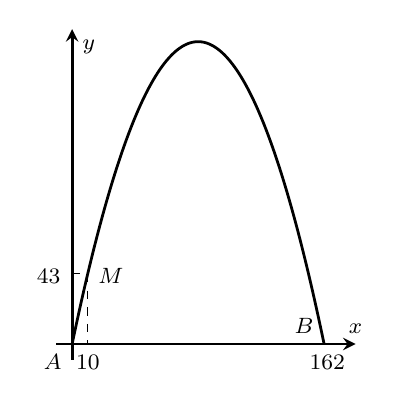
\begin{tikzpicture}[scale=0.2,line width=1pt,>=stealth,x=1mm,y=1mm]
				\draw (0,0) node[below left] {\footnotesize $A$} (10,43) node[right]{\footnotesize $M$} (160,0) node[above left]{\footnotesize $B$};
				\draw[->] (-10,0) -- (180,0) node [above] {\footnotesize$x$};
				\draw[->] (0,-10) -- (0,200) node [below right] {\footnotesize$y$};
				\foreach \x/\xtext in {10/10,162/162}
				\draw[shift={(\x,0)}] (0pt,2pt)--(0pt,-2pt) node[below] {\footnotesize $\xtext$};
				\foreach \y/\ytext in {43/43}
				\draw[shift={(0,\y)}] (2pt,0pt)--(-2pt,0pt) node[left] {\footnotesize $\ytext$};
				\draw[dashed,thin] (0,45)--(10,45)--(10,0);
				\usepgflibrary{fpu}
				\draw[smooth,samples=100,domain=0:160,/pgf/fpu,/pgf/fpu/output format=fixed] plot(\x,{-0.03*(\x)^2+4.8*(\x)});
			\end{tikzpicture}
		}
	}
\end{ex}

\begin{ex}%[0D2K3-2]%[Dự án đề kiểm tra HKII NH22-23- Phạm Phương]%[THPT CHUYÊN LAM SƠN - THANH HÓA]
	Tìm số hạng không chứa $x$ trong khai triển nhị thức Niu-tơn của $\left(\dfrac{1}{x}+x^3\right)^4$.
	\choice
	{$1$}
	{\True $4$}
	{$6$}
	{$12$}
	\loigiai{
		Số hạng tổng quát trong khai triển của $\left(\dfrac{1}{x}+x^3\right)^4$ có dạng $\mathrm{C}_4^k\,\left(\dfrac{1}{x}\right)^{4-k}\left(x^3\right)^k=\mathrm{C}_4^k\,x^{4k-4}$ $(k \in \mathbb{N},\, k \leq 4)$.\\
		Số hạng không chứa $x$ ứng với $4k-4=0 \Leftrightarrow k=1$, do đó số hạng đó là $\mathrm{C}_4^1=4$.
	}
\end{ex}

\begin{ex}%[0H4G1-6]%[Dự án đề kiểm tra HKII NH22-23- Phạm Phương]%[THPT CHUYÊN LAM SƠN - THANH HÓA]
	Trong mặt phẳng với hệ tọa độ $Oxy$, cho hai điểm $A(1;1)$, $B(4;-3)$ và đường thẳng $d\colon x-2y-1=0$. Tìm điểm $M$ thuộc $d$ có tọa độ nguyên và thỏa mãn khoảng cách từ $M$ đến đường thẳng $AB$ bằng $6$.
	\choice
	{$M(-43;-27)$}
	{$M\left(3;-\dfrac{27}{11}\right)$}
	{$M(3;7)$}
	{\True $M(7;3)$}
	\loigiai{
		Với $A(1;1)$, $B(4;-3)$, đường thẳng $AB$ có phương trình $\dfrac{x-1}{3}=\dfrac{y-1}{-4} \Leftrightarrow 4x+3y-7=0$.\\
		Do $M \in d\colon x-2y-1=0$ và $M$ có tọa độ nguyên nên $M(2t+1;t)$, $t \in \mathbb{Z}$.\\
		Ta có $\mathrm{d}(M,AB)=\dfrac{\big|4(2t+1)+3t-7\big|}{\sqrt{4^2+3^2}}=\dfrac{\big|11t-3\big|}{5}$.\\
		Theo giả thiết $\mathrm{d}(M,AB)=6 
		\Leftrightarrow \dfrac{\big|11t-3\big|}{5}=6 
		\Leftrightarrow \big|11t-3\big|=30 \Leftrightarrow t=3$ (do $t \in \mathbb{Z}$).\\
		Vậy $M(7;3)$
	}
\end{ex}

\begin{ex}%[0H4G3-3]%[Dự án đề kiểm tra HKII NH22-23- Phạm Phương]%[THPT CHUYÊN LAM SƠN - THANH HÓA]
	Cho elip $(E)\colon\dfrac{x^2}{25}+\dfrac{y^2}{9}=1$. Trong các điểm sau đây điểm nào thuộc $(E)$ mà điểm đó nhìn hai tiêu điểm $F_1$, $F_2$ của $(E)$ dưới một góc vuông.
	\choice
	{$N\left(4;-\dfrac{9}{5}\right)$}
	{$P(0;4)$}
	{\True $Q\left(\dfrac{5\sqrt{7}}{4};\dfrac{9}{4}\right)$}
	{$M(-5;0)$}
	\loigiai{
		Elip $(E)\colon\dfrac{x^2}{25}+\dfrac{y^2}{9}=1$ có $\heva{&a^2=25\\&b^2=9}$ nên $c=\sqrt{a^2-b^2}=4$.\\
		Đường tròn $(O,c)$ có phương trình $x^2+y^2=4^2$.\\
		Xét hệ phương trình $\heva{&x^2+y^2=16\\&\dfrac{x^2}{25}+\dfrac{y^2}{9}=1} \Leftrightarrow \heva{&x^2=\dfrac{175}{16}\\&y^2=\dfrac{81}{16}} 
		\Leftrightarrow \heva{&x=\pm \dfrac{5\sqrt{7}}{4}\\&y=\pm \dfrac{9}{4}.}$\\
		Như vậy các điểm $Q_i\left(\pm\dfrac{5\sqrt{7}}{4};\pm\dfrac{9}{4}\right)$, $i\in \{1;2;3;4\}$ là giao điểm của $(O,c)$ và $(E)$ nên $Q_j$ nằm trên $(E)$ và nhìn $F_1F_2$ dưới một góc vuông (do tam giác $Q_iF_1F_2$ có trung tuyến $OQ_j=c=\dfrac{F_1F_2}{2}$).
	}
\end{ex}

\begin{ex}%[0H4K2-3]%[Dự án đề kiểm tra HKII NH22-23- Phạm Phương]%[THPT CHUYÊN LAM SƠN - THANH HÓA]
	Trong mặt phẳng $Oxy$, cho đường tròn $(C)\colon (x-1)^2+(y-4)^2=4$. Phương trình tiếp tuyến với đường tròn $(C)$ song song với đường thẳng $\Delta\colon 4x-3y-2=0$ là
	\choice
	{$4x-3y-18=0$}
	{$4x-3y+18=0;4x-3y-2=0$}
	{$4x-3y-18=0;4x-3y+2=0$}
	{\True $4x-3y+18=0$}
	\loigiai{
		Đường tròn $(C)\colon (x-1)^2+(y-4)^2=4$ có tâm $I(1;4)$ và bán kính $r=2$.\\
		Tiếp tuyến $d$ của $(C)$ song song với đường thẳng $\Delta\colon 4x-3y-2=0$ có phương trình dạng
		$$d\colon 4x-3y+c=0,\; c\neq -2.$$
		Ngoài ra $\mathrm{d}(I,d)=r \Leftrightarrow \dfrac{\big|4\cdot 1-3\cdot 4+c\big|}{\sqrt{4^2+(-3)^2}}=2
		\Leftrightarrow \big|c-8\big|=10 \Leftrightarrow \hoac{&c=-2\;\;\text{(loại)}\\&c=18\;\;\text{(nhận).}}$\\
		Vậy $d\colon 4x-3y+18=0$ là tiếp tuyến cần tìm.
	}
\end{ex}

\begin{ex}%[0D3G2-6]%[Dự án đề kiểm tra HKII NH22-23- Phạm Phương]%[THPT CHUYÊN LAM SƠN - THANH HÓA]
	Gọi $S$ là tập hợp tất cả các số tự nhiên gồm $4$ chữ số khác nhau được chọn từ tập hợp $A=\{1;2;3;4;5;6\}$. Chọn ngẫu nhiên một số từ tập hợp $S$. Tính xác suất để số được chọn có $2$ chữ số chẵn và $2$ chữ số lẻ.
	\choice
	{$\dfrac{2}{5}$}
	{$\dfrac{1}{6}$}
	{\True $\dfrac{3}{5}$}
	{$\dfrac{1}{10}$}
	\loigiai{
		Từ tập $A=\{1;2;3;4;5;6\}$ ta lập được $\mathrm{A}_6^4=360$ số tự nhiên có $4$ chữ số khác nhau.\\
		Phép thử ``chọn một số trong $360$ số đó'' cho ta số phần tử không gian mẫu là $n(\Omega)=360$.\\
		Xét biến cố $X$: ``chọn được số có $2$ chữ số chẵn và $2$ chữ số lẻ''.\\
		Số kết quả thuận lợi cho $X$ là $n(X)=\mathrm{C}_3^2\cdot\mathrm{C}_3^2\cdot 4!=216$.\\
		Vậy xác suất của $X$ là $\mathrm{P}(X)=\dfrac{216}{360}=\dfrac{3}{5}$.
	}
\end{ex}

\begin{ex}%[0D4G2-1]%[Dự án đề kiểm tra HKII NH22-23- Phạm Phương]%[THPT CHUYÊN LAM SƠN - THANH HÓA]
	Tìm số các giá trị nguyên của tham số $m \in [-10;10]$ để bất phương trình $\dfrac{3x^2-(m+6)x+12}{4x^2-5x+8}>0$ nghiệm đúng với mọi giá trị $x \in \mathbb{R}$.
	\choice
	{$18$}
	{$15$}
	{$14$}
	{\True $16$}
	\loigiai{
		Do $4x^2-5x+8$ vô nghiệm và có hệ số của $x^2$ bằng $4>0$ nên $4x^2-5x+8>0,\;\forall x \in \mathbb{R}$.\\
		Từ đó $\dfrac{3x^2-(m+6)x+12}{4x^2-5x+8}>0$ nghiệm đúng với mọi $x \in \mathbb{R}$ khi và chỉ khi 
		\allowdisplaybreaks
		$$\begin{aligned}
			3x^2-(m+6)x+12>0,\;\forall x \in \mathbb{R}
			&\Leftrightarrow \Delta=(m+6)^2-4\cdot3\cdot 12<0 \text{ (do } a=3>0)\\
			& \Leftrightarrow m^2+12m-108<0\\
			& \Leftrightarrow -18<m<6.
		\end{aligned}$$
		Xét $m \in \mathbb{Z} \cap [-10;10]$ ta nhận $m \in \{-10;-9;\ldots;4;5\}$ (có $16$ giá trị $m$).
	}
\end{ex}

\begin{ex}%[0H4G2-5]%[Dự án đề kiểm tra HKII NH22-23- Phạm Phương]%[THPT CHUYÊN LAM SƠN - THANH HÓA]
	Trong mặt phẳng tọa độ $Oxy$, cho đường tròn $(C)\colon x^2+y^2-2x-4y-25=0$ và điểm $M(2;1)$. Dây cung của $(C)$ đi qua $M$ có độ dài ngắn nhất là
	\choice
	{\True $4\sqrt{7}$}
	{$8\sqrt{2}$}
	{$16\sqrt{2}$}
	{$2\sqrt{7}$}
	\loigiai{
		Đường tròn $(C)\colon x^2+y^2-2x-4y-25=0$ có tâm $I(1;2)$ và bán kính $r=\sqrt{1^2+2^2-(-25)}=\sqrt{30}$.
		\immini{
			Do $IM=\sqrt{1^2+(-1)^2}=\sqrt{2}<r$ nên $M$ nằm bên trong đường tròn $(C)$.\\
			Xét dây cung $AB$ đi qua $M$, với $A,B \in (C)$ và $H$ là trung điểm của $AB$.\\
			Khi đó $\heva{&H \text{ là hình chiếu của }I \text{ lên }AB\\&M \text{ thuộc } AB}$ nên $IH \leq IM$.
			\begin{center}
				(dấu ``$=$'' xảy ra khi và chỉ khi $H \equiv M$)
			\end{center}
			Và $AB=2AH=2\sqrt{r^2-IH^2} \geq 2\sqrt{30-IM^2}=2\sqrt{30-2}=4\sqrt{7}$.
			\begin{center}
				(dấu ``$=$'' xảy ra khi và chỉ khi $H \equiv M$)
			\end{center}
			}
		{\vspace{0.1cm}
			\begin{tikzpicture}[scale=0.95, font=\footnotesize, line join=round, line cap=round]
				\coordinate (I) at (0,0);
				\coordinate (A) at (-150:2);
				\coordinate (B) at (-30:2);
				\coordinate (H) at ($(A)!1/2!(B)$);
				\coordinate (M) at ($(A)!0.33!(B)$);
				\draw (I) circle (1pt) node[above]{$I$};
				\draw (A) circle (1pt) node[below left=-3pt]{$A$};
				\draw (B) circle (1pt) node[below right=-3pt]{$B$};
				\draw (M) circle (1pt) node[below]{$M$};
				\draw (H) circle (1pt) node[below]{$H$};
				\draw (0,0) circle (2);
				\draw (I)--(A)--(B) (M)--(I)--(H);
		\end{tikzpicture}}
	Vậy dây cung của $(C)$ đi qua $M$ có độ dài ngắn nhất là $\min_{AB}=4\sqrt{7}$.
	}
\end{ex}


\Closesolutionfile{ans}
%\begin{center}
%	\textbf{ĐÁP ÁN}
%	\inputansbox{10}{ans/ans}	
%\end{center}
